% Charlotte Geiger - Manuel Lippert - Leonard Schatt
% Physikalisches Praktikum

% Teilauswertung 2

\section{Ausgangskennlinie des Transistors}
Um die Ausgangskennlinie zu skizzieren verwenden wir die Bilder des Oszilloskops (Kapitel \ref{sec:zusatz}: Zusatz) und nehmen an, dass außerhalb der Anzeige des Oszilloskops die Linie linear fortgeführt werden kann. 
\begin{center}
    \captionof{figure}{$U_{BE}-I_C$ Diagramm - Ausgangskennlinie Transistor}
    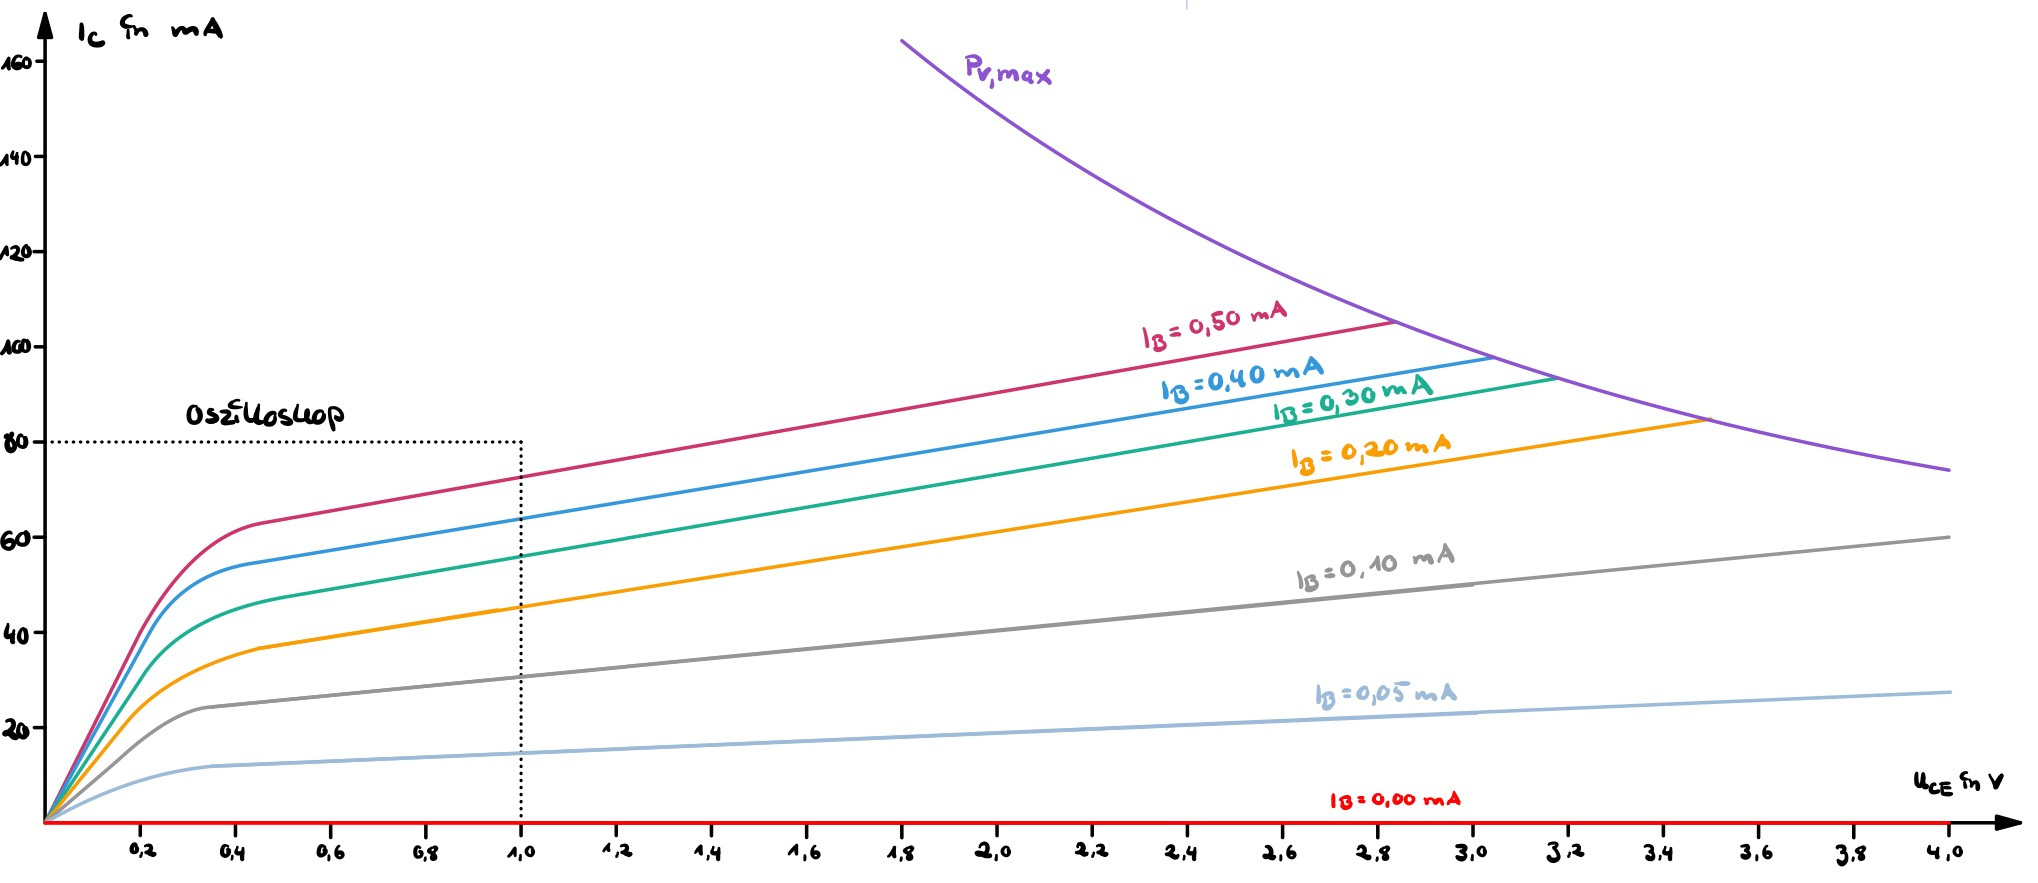
\includegraphics[scale=0.2]{6_2-Ausgangskennlinien.PNG}
\end{center}
Wobei die Datenpunkte für $P_{\text{v,max}}$-Kurve so berechnet wurden, dass für unterschiedliche $U_{CE}$ die maximale Kollektorstrom $I_C$ berechnet wurden mit
\begin{align}
    I_C=\frac{P_{\text{v,max}}}{U_{CE}} \tab\text{mit}~P_{\text{v,max}}=300~\text{mW}
\end{align}
\begin{center}
    \captionof{table}{$P_{\text{v,max}}$-Kurve}
    \begin{tabular}{l|rrrrrrrrrrrr}
        $U_{CE}/\text{V}$ & 1.8   & 2     & 2.2   & 2.4   & 2.6   & 2.8   & 3     & 3.2   & 3.4   & 3.6   & 3.8   & 4 \\
        \hline
        $I_C/\text{mA}$  & 167 & 150 & 136 & 125 & 115 & 107 & 100 & 94 & 88 & 83 & 79 & 75 \\
    \end{tabular}
\end{center}
Bei Interpretation der Graphik im Ausschnitt des Oszilloskops fallen verschiedene Punkte auf. Das zentralste Augenmerk der Grafik ist die \"ahnliche x-Koordinate des "Knicks", die bei allen ungef\"ahr bei 3,5 Volt liegt. Zus\"atzlich bemerkt man, dass alle Kennlinien ab da recht linear sind, jedoch bei steigendem Basisstrom mit gr\"o\ss{}erer Steigung.
Zudem sollen wir den differentiellen Transistor-Ausgangswiderstand mit zunehmendem Basisstrom betrachtet werden.
\begin{equation}
r_{CE}=\frac{\partial{U_{CE}}}{\partial{I_C}}\Bigg|_{I_B=const}
\end{equation}
Bei Betrachtung der Werte wird auff\"allig, dass bei konstantem $I_C$ und bei steigendem $I_B$ der Wert von $r_{CE}$ f\"allt. Daher wird deutlich, dass die Beziehung $r_{CE}\sim \frac{1}{I_B}$ gilt.\\\\
Zuletzt sollen wir noch die DC-Verst\"arkung $B=\frac{I_C}{I_B}$ berechnen. Dafür lesen wir $I_C$ für eine feste Spannung $U_{CE}=0.6~\text{V}$ aus den Bilder des Oszilloskops. Dabei wird $U_{CE}$ so gewählt, dass $I_C$ im linearen Bereich der Ausgangskennlinie beim Arbeitspunkt abgelesen wird. Weiterhin nehmen wir einen großzügigen Fehler für $I_C$ von $s_{I_C}=2.5~\text{mA}$ an, also ein halbes Kästchen auf dem Oszilloskop.  Daraus folgt:
\begin{align}
    s_B=\frac{s_{I_C}}{I_B}
\end{align}
Der Fehler des Basisstroms $s_{I_B}$ wird vernachlässigt, da dieser klein gegenüber den gewählten Fehler $s_{I_C}$ ist und damit vernachlässigbar.
\begin{center}
    \captionof{table}{DC-Verstärkung}
    \begin{tabular}{ccc|cc}
        $I_B/\text{mA}$ & $I_C/\text{mA}$ & $s_{I_C}/\text{mA}$ & $B$ & $s_B$ \\
        \hline
        0     & 0     & -   & -   & - \\
        0.05  & 13    & 2.5   & 260   & 50 \\
        0.10   & 27    & 2.5   & 270   & 25 \\
        0.20   & 39    & 2.5   & 195   & 12.5 \\
        0.30   & 49    & 2.5   & 163   & 8 \\
        0.40   & 58    & 2.5   & 145   & 6 \\
        0.50   & 63    & 2.5   & 126   & 5 \\
        \end{tabular}
\end{center}
\begin{center}
    \captionof{figure}{$I_B-B$ Diagramm}
    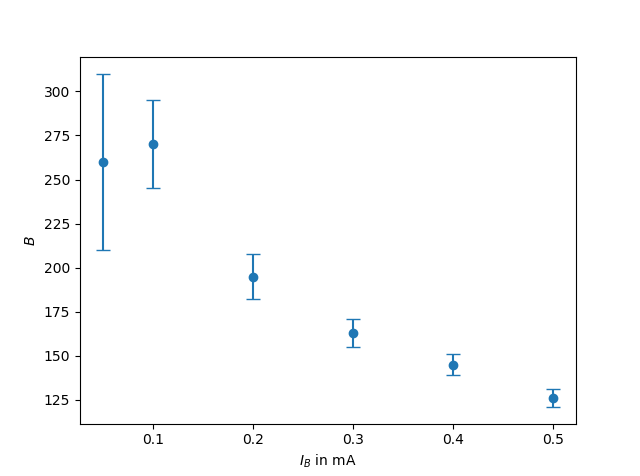
\includegraphics[scale=0.6]{6_2-Verstaerkung.png}
\end{center}
Aus dieser Abbildung kann man einen Graph erahnen, der zuerst ansteigt, jedoch dann immer schw\"acher abf\"allt. Dieses Ph\"anomen best\"atigt die Theorie, dass wie auch beim Ausgangswiderstand auch die Verst\"arkung mit zunehmendem Basisstrom abf\"allt. \\